\documentclass{article}
\usepackage{graphicx}
\title{COMP24412 Lab 3 - The Riddle of Steel Report}
\author{Tejas Chandrasekar}
\begin{document}
\maketitle
\newpage

\section{Lexical Analysis}
Steel is alloy of iron and carbon, and sometimes other elements. Because of
its high tensile strength and low cost, it is a major component used in
buildings, infrastructure, tools, ships, automobiles, machines, appliances, and
weapons.\par
\begin{enumerate}
  \item POS tagging the above sentence:
  \begin{itemize}
    \item NN: Noun, singular or mass
    \begin{itemize}
      \item steel
      \item alloy
      \item iron
      \item carbon
      \item strength
      \item cost
      \item component
      \item infrastructure
    \end{itemize}
    \item NNS: Noun, plural
    \begin{itemize}
      \item elements
      \item buildings
      \item tools
      \item ships
      \item automobiles
      \item machines
      \item appliances
      \item weapons
    \end{itemize}
    \item JJ: Adjectives
    \begin{itemize}
      \item other
      \item high
      \item tensile
      \item low
      \item major
    \end{itemize}
    \item RB: Adverb
    \begin{itemize}
      \item sometimes
    \end{itemize}
    \item CC: Coordinating conjunction
    \begin{itemize}
      \item Because
      \item and
    \end{itemize}
    \item DT: Determiner
    \begin{itemize}
      \item an
      \item a
      \item its
    \end{itemize}
    \item IN: Preposition/subordinating conjunction
    \begin{itemize}
      \item in
      \item of
    \end{itemize}
    \item VBD: Verb, past tense
    \begin{itemize}
      \item Used
    \end{itemize}
    \item VZD: Verb, 3rd person singular present
    \begin{itemize}
      \item is
    \end{itemize}
    \item PP\$: Possessive pronoun
    \begin{itemize}
      \item it
    \end{itemize}
  \end{itemize}
  \item Pronominal co-references: steel, it
\end{enumerate}

\section{C-Structures}
Sentence is 'Steel is an alloy of iron and carbon, and sometimes other
elements.'.
\begin{enumerate}
  \item Constituency structure:
  \begin{figure}
    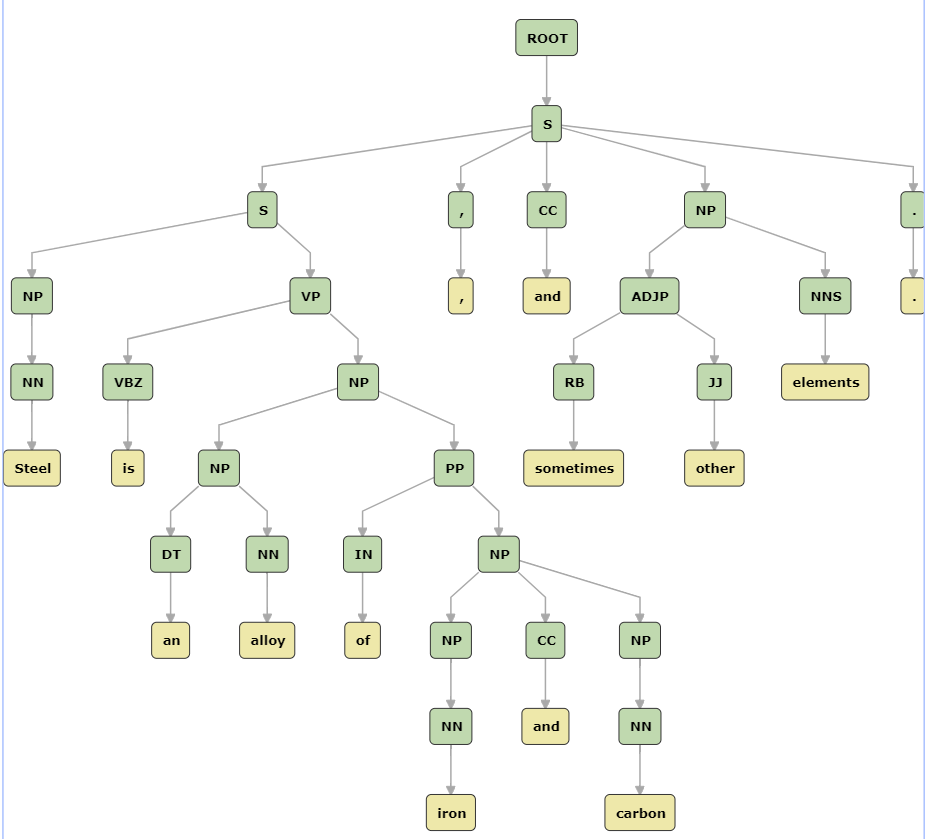
\includegraphics[width=\linewidth]{task2img.PNG}
    \caption{C-strcuture for the sentence}
    \label{Cstruct}
  \end{figure}
  \item Nominal phrasal nodes:
  \item Co-ordinations:
  \begin{itemize}
    \item Coordinating conjunction: '...iron AND carbon, AND...'
    \item Gapped coordination: '...sometimes other elements.'
  \end{itemize}
\end{enumerate}

\end{document}
